% -----------------------------------------------
% Template for ISMIR Papers
% 2019 version, based on previous ISMIR templates

% Requirements :
% * 6+n page length maximum
% * 4MB maximum file size
% * Copyright note must appear in the bottom left corner of first page
% * Clearer statement about citing own work in anonymized submission
% (see conference website for additional details)
% -----------------------------------------------

\documentclass{article}
\usepackage[T1]{fontenc} % add special characters (e.g., umlaute)
\usepackage[utf8]{inputenc} % set utf-8 as default input encoding

% TADY BUĎ MIREX2010 NEBO ISMIR
\usepackage{ismir,amsmath,cite,url}
% \usepackage{mirex2010,amsmath,cite,url}
\usepackage{graphicx}
\usepackage{color}

\usepackage{booktabs}       % lepší vodorovné linky v tabulkách
\usepackage{xcolor}
\usepackage{colortbl}


% Optional: To use hyperref, uncomment the following.
% \usepackage[bookmarks=false,hidelinks]{hyperref}
% Mind the bookmarks=false option; bookmarks are incompatible with ismir.sty.

% Title.
% ------
\title{Melody Extraction using a Harmonic Harmonic Convolutional Neural Network}

% Note: Please do NOT use \thanks or a \footnote in any of the author markup

% Single address
% To use with only one author or several with the same address
% ---------------
%\oneauthor
% {Names should be omitted for double-blind reviewing}
% {Affiliations should be omitted for double-blind reviewing}

% Two addresses
% --------------
\twoauthors
 {Jiří Balhar} {Charles University \\ Institute of Formal and Applied Linguistics \\ {\tt balhar.j@gmail.com}}
 {Jan Hajič jr.} {Charles University \\ Institute of Formal and Applied Linguistics \\ {\tt hajicj@ufal.mff.cuni.cz}}

%% To make customize author list in Creative Common license, uncomment and customize the next line
%  \def\authorname{First Author, Second Author}

\sloppy % please retain sloppy command for improved formatting

\begin{document}

%
\maketitle
%
\begin{abstract}
Melody extraction is arguably one of the most challenging and potentially rewarding problems in Music Information Retrieval. It is melody that we are likely to recall after listening to a song and so it is one of the most relevant aspects of music. However the presence of accompaniment in songs makes the task hard to address using rule-based methods. During the last years data-driven methods based on deep learning started to outperform methods traditionally used in the field. In this paper we continue in these efforts and propose a new method for melody extraction. An architecture called \emph{Harmonic Convolutional Neural Network}, based on a modification of convolutional neural networks to better capture harmonically related information in an input spectrogram with logarithmic frequency axis, was able to achieve state-of-the-art performance on most publicly available melody datasets.
\end{abstract}
%
\section{Introduction}\label{sec:introduction}
% inspirace:
% https://www.music-ir.org/mirex//abstracts/2016/KON1.pdf
% https://www.music-ir.org/mirex//abstracts/2016/BG1.pdf
% 2-3 stránky!!

In the recent years the approaches to melody extraction have shifted from signal processing, rule-based methods and statistical modeling using HMMs \cite{Salamon2014} to the use of deep learning (DL). The task is being framed as a standard classification problem \cite{Poliner,Kum2016,Rigaud2016,Balke2017,DBasaranSEssid2018} or as a de-noising problem \cite{Bittner2017}. In general these new methods operate in two steps. First they transform the input signal to a time-frequency representation (STFT, CQT, $H^{F_0}$) and then use machine learning methods such as convolutional neural network (CNN) to sequentially process the transformed input. The result is a saliency map from which they select the melody $f_0$ trajectory and determine voicing.

Among new DL-based works we can find variety of approaches that focus on different input signal transformations, network topologies and postprocessing techniques. On the other hand the building blocks out of which these systems are built are standard (fully connected layers, CNNs and RNNs). In this paper we propose a new kind of CNN architecture specialized for processing harmonic signals in audio. % We base our method on the work of Bittner et al. \cite{Bittner2017}. 
\footnote{For the source code please see the accompanying repository at \url{https://github.com/kukas/music-transcription}}

\subsection{The use of CNNs for Melody Extraction}

A harmonic signal of fundamental frequency $f_0$ can be viewed as a weighted sum of harmonically related sinusoids. A time-frequency representation of this kind of signal therefore exhibits peaks at these frequencies. Since a melody in a song recording is almost always a harmonic signal, using this property of a harmonic signal was the basis for Melody Extraction systems before the shift to DL \cite{Salamon2014}.

The use of CNNs on input time-frequency representations has a major limitation in this context. CNN kernels are usually small (previous works use usually a size of a semitone in the frequency axis \cite{Bittner2017,DBasaranSEssid2018}) and therefore cannot process the whole harmonic structure in one layer. When using a small kernel, any output value depends only on the nearest input values and this "receptive field" scales only linearly with the number of layers. To make up for this, existing networks also include a final "big" convolutional layer to "capture relationships between frequency content withing a octave" \cite{Bittner2017}. This is only a partial solution because only one layer of the whole network can exploit the defining characteristic of a harmonic signal. There is also the additional drawback of adding a large number of potentially unnecessary parameters to the network (since the layer needs to capture only the harmonics) which is a concern in Melody Extraction task since training data available is scarce.


\begin{figure}
 \centerline{\framebox{
 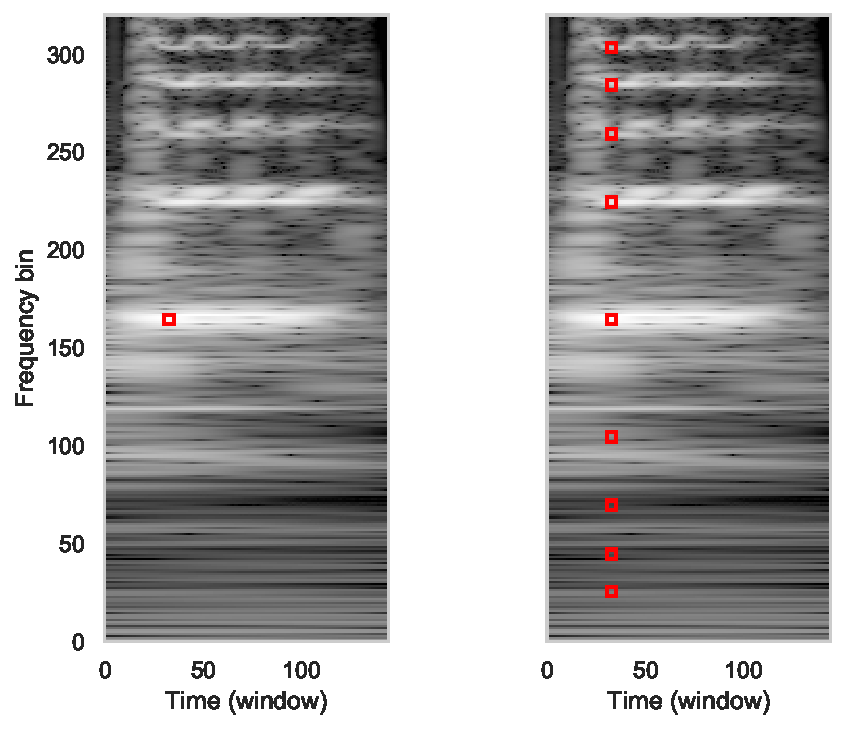
\includegraphics[width=\columnwidth]{vibrato}}}
 \caption{Comparison of receptive fields of standard CNN and HCNN on a CQT spectrogram.}
 \label{fig:vibrato}
\end{figure}

\section{Method}\label{sec:method}

Our proposed Harmonic Convolutional Neural Network (HCNN) overcomes the limitation outlined in the Introduction. The convolutional layer in our network is able to use all the relevant harmonic information in each layer as illustrated in \figref{fig:vibrato}. 

The architecture has the standard overall structure of processing an input through a series of convolutional layers. We use only convolutions with 1x1 stride and no pooling layers so that the input and output sizes stay the same throughout the whole network. The output of each layer is therefore a 3D matrix with channel, frequency and time axes of constant dimensions. Crucially before processing each convolutional layer we apply an additional transformation of the input to each layer (see \figref{fig:hcnn_transform}). 

The transformation first creates copies of the input and stacks them in the channel axis, so that there are several identical copies of the input matrix. We then shift those copies relative to the original in the frequency axis so that the information about harmonically related peaks are positioned "above"\footnote{"above" meant in the channel axis} the original fundamental frequency. Since the input is a log-frequency spectrogram, the offsets are constant. For example in our case the shift of $60$ bins corresponds to an octave (second harmonic frequency) and the shift of $60+35$ bins corresponds to an octave and a fifth (third harmonic frequency). In this way we can position as many harmonically related bins on top of each other as needed. 

In addition to the shift to corresponding overtones, we also add copies shifted in the opposite direction. This allows the convolution to access corresponding fundamental frequency values when processing some of the overtones of a harmonic signal. We call those negative offsets "undertones".

This transformed input is then fed into the next convolutional layer. Since the convolutional filter has the access to all channels, it follows that it has access to the provided harmonically related information for every time-frequency position in the matrix.

\begin{figure}
 \centerline{\framebox{
 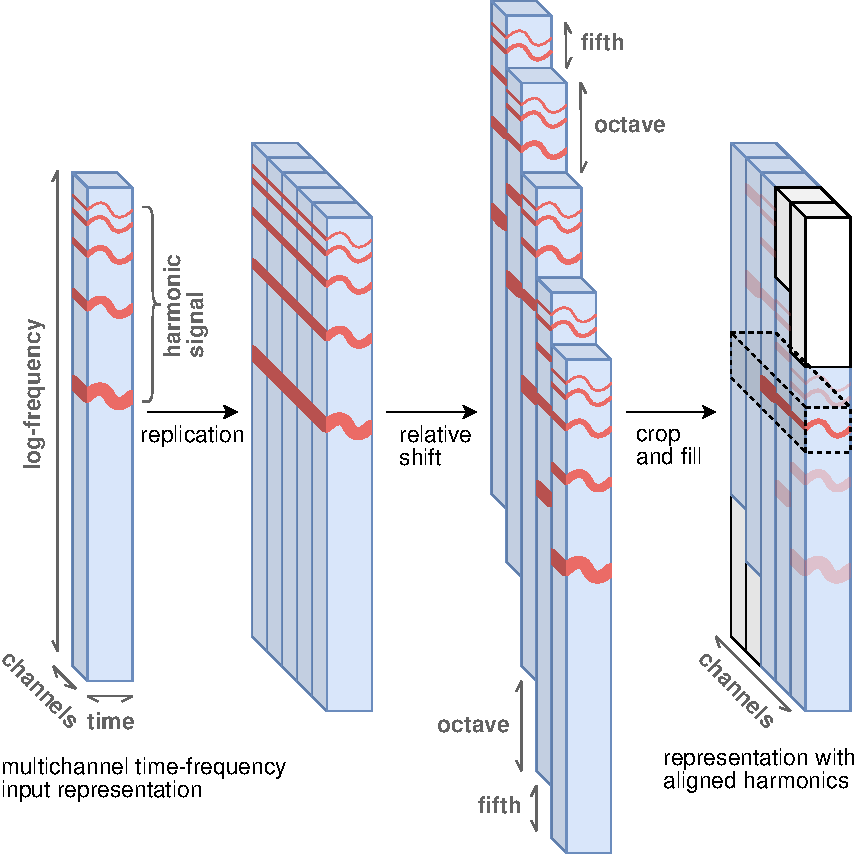
\includegraphics[width=\columnwidth]{hcnn_transform_en_2}}}
 \caption{Diagram of the input transformation for convolution layers.}
 \label{fig:hcnn_transform}
\end{figure}

\subsection{Input representation}

The input is a single CQT spectrogram with 5 bins per semitone and 540 bins in total (spanning the range from C1 to C9). Our hop size is $\frac{256}{44100} \approx 5.8\,\rm ms$. Note that CQT has logarithmically spaced frequency bins, which is an essential property for our method to work because it implies that distances between the harmonics are independent on the fundamental frequency of a signal. By applying the harmonic-alignment transformation explained in the previous section to this CQT input, we create a 3-dimensional array that closely resembles HCQT input representation used in \cite{Bittner2017} without the overhead of computing each CQT spectrogram separately. This allows us to cheaply increase the number of HCQT harmonics. We therefore create a HCQT representation by stacking 8 copies shifted by overtone offsets and 8 copies shifted by undertone offsets. Finally we crop the HCQT to match the output dimensions (360 bins, range from C1 to C6).

\subsection{Output representation}

The output representation matches the cropped input frequency and time dimensions. In each timeframe the ground truth is represented as a gaussian with mean in the reference $f_0$ and standard deviation of 18 cents. Unvoiced frames are represented as zero vectors. Voicing output is obtained by thresholding the maximum value of each frame using a best performing threshold for the validation dataset. This representation is inspired by CREPE monopitch tracker \cite{Kim2018}, the std. dev. was finetuned for our purposes.


\begin{figure}
 \centerline{\framebox{
 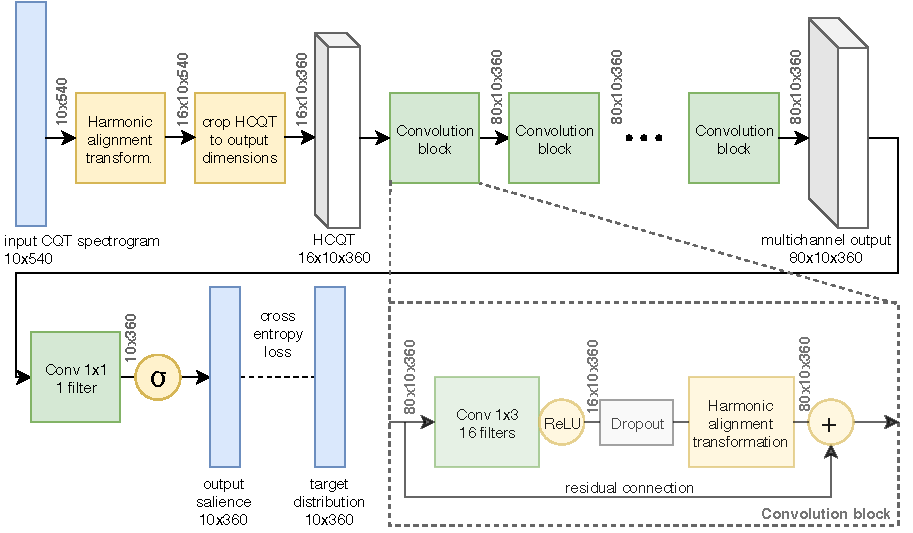
\includegraphics[width=\columnwidth]{hcnn_overall_2}}}
 \caption{Overall HCNN architecture.}
 \label{fig:hcnn_overall}
\end{figure}

% \begin{figure}
%  \centerline{\framebox{
%  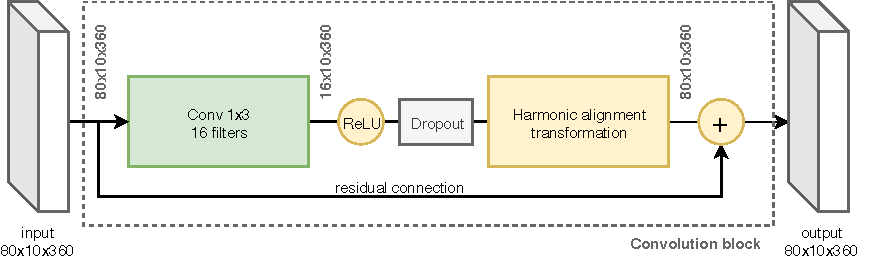
\includegraphics[width=\columnwidth]{hcnn_convblock_2}}}
%  \caption{Convolution block.}
%  \label{fig:hcnn_convblock}
% \end{figure}

\begin{figure}
 \centerline{\framebox{
 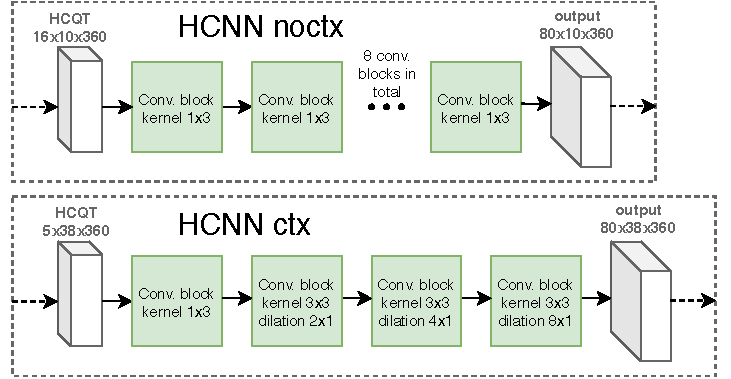
\includegraphics[width=\columnwidth]{hcnn_archs_2}}}
 \caption{Two tested architectures.}
 \label{fig:hcnn_archs}
\end{figure}

\subsection{Architecture}

The design of the rest of the network either draws from standard deep learning practices and from Bittner et al. \cite{Bittner2017} (see \figref{fig:hcnn_overall}). The input HCQT is processed using a stack of convolution blocks. The output is passed through a 1x1 convolution to shrink the number of channels and create a salience representation. The model is trained using cross entropy loss using Adam optimizer with learning rate 0.001 and 16 samples per batch.

A convolution block consists of a convolutional layer with 16 filters and ReLU activation, followed by a dropout layer (with dropout probability of 0.3) and the harmonic alignment transformation. We also add a residual connection \cite{He2015} as it improves the model performance with no significant additional overhead.

We test two architectures, HCNN noctx and HCNN ctx. HCNN noctx consists of 8 convolution blocks that contain convolutional layers with kernel size 3x1. In other words the convolutions operate only in the frequency dimension and thus the estimation is based only on one frame of the input spectrogram ($\approx 5.8\,\rm ms$ of audio). The harmonic aligment transformation for this architecture includes the first two undertones and overtones (channels shifted by -19, -12, 0, 12 and 19 semitones).

The HCNN ctx architecture consists of 4 convolution blocks. The first block with kernel size 3x1 and the rest with sizes 3x3. Additionaly we set an increasing dilation rate in the last three convolution blocks (along the lines of the WaveNet architecture \cite{Oord2016}). In this way we achieve a receptive field of $\approx 162.4\,\rm ms$ using only three layers that operate also in the time dimension. Note that this resulting receptive field is comparable to Bittner et al. \cite{Bittner2017}.

\begin{table}
\centering
\scalebox{1.0}{%
\begin{tabular}{lrrrrrr}
\toprule
Method & Parameters \\
\midrule
    SAL &         ---   \\
    BIT &         406 253 \\
    BAS &         307 199 \\
\arrayrulecolor{black!30}\midrule
 HCNN noctx & 27 857 \\
 HCNN ctx   & 23 153 \\
\arrayrulecolor{black}\bottomrule
\end{tabular}
}%
\caption{Comparison of the number of model parameters.}\label{tab:model_parametes}
\end{table}

\section{Experiments}

\subsection{Datasets}

For training and validation, we use MedleyDB \cite{Bittner2014}. We use the same dataset split as in \cite{DBasaranSEssid2018,Bittner2017}. This has the advantage of being able to directly compare the results of the methods on the testing split. 

Besides the MedleyDB testing set, for testing we also include ADC04 dataset, MIREX05 training set \footnote{We downloaded ADC04 and MIREX05 datasets from \url{https://labrosa.ee.columbia.edu/projects/melody/}}, Orchset \cite{Bosch2016}, a subset of MDB-melody-synth \cite{Salamon2017} and a subset of WJAZZD \cite{Pfleiderer}. \footnote{For the complete list of selected testing tracks please see the repository at \url{https://github.com/kukas/music-transcription}.}

\subsection{Methodology}

For evaluation, we use the melody extraction evaluation functions from the library \texttt{mir\_eval}\footnote{\url{https://github.com/craffel/mir_eval}}. These include the standard metrics used in the context of Melody Extraction. We compare the output of our models "HCNN noctx" (HCNN with minimal audio context) and "HCNN ctx" (HCNN with broader audio context) with state-of-the-art baselines: "SAL" \cite{Salamon2012a}, "BIT" \cite{Bittner2017} and "BAS" \cite{DBasaranSEssid2018}. In case of BIT and BAS, we ran the algorithms using the source code obtained from the links provided in the papers keeping default parameters. For the SAL algorithm we used the implementation in Essentia library \footnote{\url{https://essentia.upf.edu}}. All the output melody estimates are included in the repository.

% \subsection{Harmonic Convolutional Neural Network}

\begin{figure}
 \centerline{\framebox{
 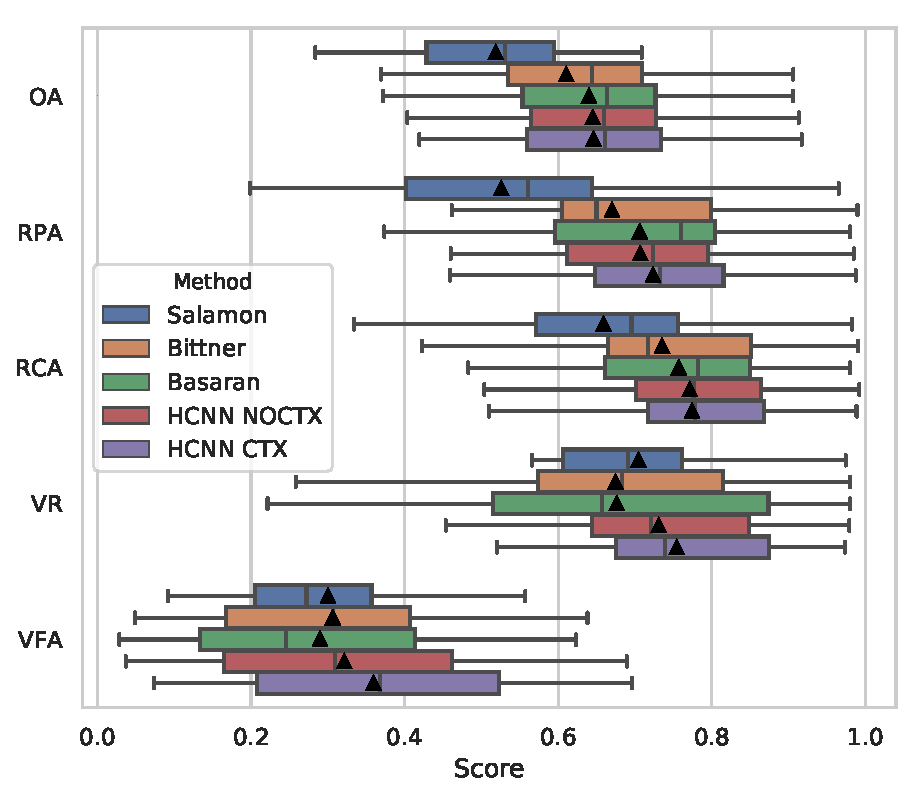
\includegraphics[width=\columnwidth]{medleydb_scores_sota}}}
 \caption{Evaluation metrics on MedleyDB testing split for SAL, BIT, BAS, HCNN noctx and HCNN ctx.}
 \label{fig:medleydb_scores_sota}
\end{figure}


\begin{table}
\centering
\scalebox{0.75}{%
\begin{tabular}{lrrrrrr}
\toprule
Method & ADC04 & \shortstack[r]{MDB-m-s\\ test} & \shortstack[r]{MIREX05\\train.} & \shortstack[r]{MDB\\test} & \shortstack[r]{ORCH-\\SET} & \shortstack[r]{WJazzD\\test} \\
\midrule
    SAL &         0.714 &           0.527 &          0.715 &         0.519 &        0.235 &        0.667 \\
    BIT &         0.716 &           0.633 &          0.702 &         0.611 &        0.407 &        0.692 \\
    BAS &         0.669 &   \textbf{0.689}&          0.734 &         0.640 &\textbf{0.483}&        0.700 \\
\arrayrulecolor{black!30}\midrule
 \shortstack[l]{HCNN\\ noctx} & \textbf{0.737}&           0.626 &          0.723 &         0.635 &        0.439 &        0.715 \\
 \shortstack[l]{HCNN\\ ctx}   &         0.726 &           0.661 &  \textbf{0.755}& \textbf{0.652}&        0.459 &\textbf{0.725} \\
\arrayrulecolor{black}\bottomrule
\end{tabular}
}%
\caption{Overall Accuracy of the selected methods. Highlighted values are the highest across the dataset.}\label{tab:results_OA}
\end{table}

\subsection{Results}\label{sec:results}

\textcolor{red}{Trochu rozepsat a kvantitativní obrázek}

We present a detailed comparison of the results of the selected methods on MedleyDB testing split on \figref{fig:medleydb_scores_sota} and a overview of Overall Accuracy on six different datasets in \tabref{tab:results_OA}. Our methods outperform all selected baselines on four out of six testing datasets. Compared to the most similar method of Bittner et al. \cite{Bittner2017} we achieve better results on all datasets with a gain of +3.6 percentage points in average on the Overall Accuracy (OA) metric. Basaran et al. \cite{DBasaranSEssid2018}, who additionally use a recurrent layer on top of the convolutional stack, therefore giving the network an advantage over the HCNN and Bittner by allowing it to learn also how melody works in time, comes much closer with a +1.0 average percentage point difference. Compared to the methods based on deep learning (Bittner and Basaran), our model uses between 10 and 20 times less parameters (see \tabref{tab:model_parametes}).

Qualitatively we see an expected difference between the outputs of HCNN noctx, HCNN ctx and BAS. The results of HCNN noctx are noisier compared to HCNN ctx and BAS, since one audio input frame is only $5.8\,\rm ms$ long. It is impossible for this method to take into account any musical context even within one continuous note. For pieces with higher polyphony, the output of HCNN noctx therefore jumps between possible melody $f_0$ candidates.

The results of HCNN ctx and Bittner are highly correlated, from a closer qualitative inspection we conclude that the performance difference can be attributed to a better generalization on instrument classes underrepresented in the training dataset and better learning of the instrument priorities.

\section{Conclusion}

In this paper we presented a novel and general way to adapt ordinary CNN-based networks for processing harmonic audio signals. We showed that using HCNN layers is effective for the Melody Extraction task and yields state-of-the-art results while dramatically reducing the needed number of parameters of the model. Based on these results we believe that the architecture has a potential in other related tasks such as multi-$f_0$ tracking.
%HCNNs might be also applicable in speech-recognition tasks, since human speech is also a harmonic signal. 
The small size of the model also allows for inference without a dedicated GPU opening the potential for use in mobile devices or low-end PCs.

Possible improvements include data augmentation (see \cite{Park_2019} for an interesting new data augmentation technique designed for audio data) and temporal smoothing of the output using HMM, LSTM or other techniques like in Basaran et al. \cite{DBasaranSEssid2018}. Other potential improvements can be done by altering the input representation or the model architecture. 


% For bibtex users:
\bibliography{library}

\end{document}
